\documentclass[border=10pt]{standalone}
\usepackage{pgfplots}
\pgfplotsset{compat=1.18}

\begin{document}
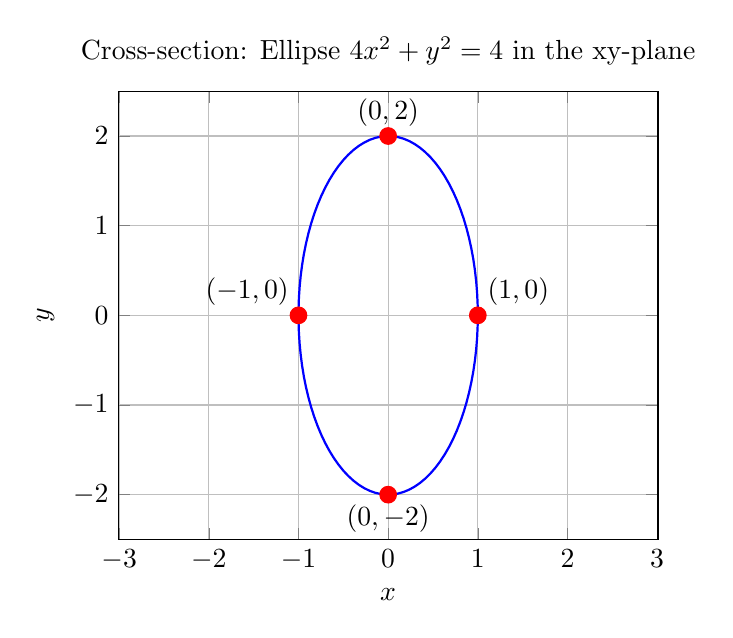
\begin{tikzpicture}
\begin{axis}[
    xlabel={$x$},
    ylabel={$y$},
    title={Cross-section: Ellipse $4x^2 + y^2 = 4$ in the xy-plane},
    axis equal,
    grid=major,
    xmin=-2.5, xmax=2.5,
    ymin=-2.5, ymax=2.5,
    ]
    
    % Plot the ellipse using parametric equations
    \addplot[
        domain=0:360,
        samples=100,
        thick,
        blue,
    ]
    ({cos(x)}, {2*sin(x)});
    
    % Mark the intercepts
    \addplot[only marks, red, mark=*, mark size=3pt] 
        coordinates {(1,0) (-1,0) (0,2) (0,-2)};
    
    % Add labels for intercepts
    \node[anchor=south west] at (axis cs:1,0) {$(1, 0)$};
    \node[anchor=south east] at (axis cs:-1,0) {$(-1, 0)$};
    \node[anchor=south] at (axis cs:0,2) {$(0, 2)$};
    \node[anchor=north] at (axis cs:0,-2) {$(0, -2)$};
    
\end{axis}
\end{tikzpicture}
\end{document}